\documentclass[11pt,a4paper]{article}

\usepackage[utf8]{inputenc}
\usepackage[T1]{fontenc}
% Espanol portable: si babel-spanish no esta instalado como .ldf, se carga
% via el archivo locale ini (babelprovide). Si en tu maquina tenes el paquete
% completo, pod\'es reemplazar estas dos lineas por:
%     \usepackage[spanish,es-noquoting]{babel}
\usepackage{babel}
\babelprovide[import, main]{spanish}
\usepackage{amsmath,amssymb}
\usepackage{graphicx}
\usepackage[margin=2.5cm]{geometry}
\usepackage{booktabs}
\usepackage{siunitx}
\usepackage{xcolor}
\usepackage[colorlinks=true,linkcolor=blue,citecolor=blue,urlcolor=blue]{hyperref}

% Atajos
\newcommand{\mchi}{m_\chi}
\newcommand{\eps}{\varepsilon}
\newcommand{\Ek}{E_k}
\newcommand{\Ekz}{E_k^0}
\newcommand{\cosz}{\cos\theta_k^0}
\newcommand{\gammastar}{\gamma^\ast}
\newcommand{\Phip}{\Phi_p}
\newcommand{\dd}{\mathrm{d}}
\newcommand{\Du}{\texttt{[Du]}}
\newcommand{\LZ}{\texttt{[LZ]}}

\title{\textbf{Implementaci\'on del canal de \emph{proton bremsstrahlung} (PB)\\
para el flujo atmosf\'erico de part\'iculas milicargadas}\\[4pt]
\large Generador del \emph{splitting kernel} de Du, Fang \& Liu y validaci\'on
contra LUX-ZEPLIN}
\author{Proyecto mCP --- \texttt{mCP\_from\_the\_Heaven}}
\date{\today}

\begin{document}
\maketitle

\begin{abstract}
Se documenta la implementaci\'on desde cero del canal de producci\'on de
part\'iculas milicargadas (mCP) por \emph{proton bremsstrahlung} (PB) en la
atm\'osfera, siguiendo el ``new method'' de Du, Fang \& Liu
(\href{https://arxiv.org/abs/2211.11469}{arXiv:2211.11469}, en adelante \Du).
El desarrollo se estructura en dos m\'odulos de Python: uno que genera el
\emph{splitting kernel} $p\to\gammastar p$ junto con los form factors
vectorial y off-shell, y otro que monta sobre \'el la secci\'on eficaz, la
multiplicidad por interacci\'on y el flujo de superficie. Como validaci\'on
del kernel se reproduce la Fig.~5 de \Du; como \emph{sanity check} global se
reproduce la curva de flujo PB del panel superior de la Fig.~1 de LUX-ZEPLIN
(\href{https://arxiv.org/abs/2412.04854}{arXiv:2412.04854}, en adelante \LZ),
que adopta precisamente el flujo de \Du. Se recuperan las tres
caracter\'isticas de esa curva --- meseta a baja masa, el codo en
$\mchi=m_\rho/2$ y la ca\'ida abrupta --- con la normalizaci\'on correcta en
orden de magnitud.
\end{abstract}

\tableofcontents

% ============================================================
\section{Objetivo y contexto}
% ============================================================

El proyecto calcula la sensibilidad de un detector tipo SENSEI (Skipper-CCD
de silicio) en SNOLAB a mCP atmosf\'ericas. Hasta ahora el flujo consideraba
s\'olo el canal de decaimiento de mesones (MD), a partir del formalismo de
Arg\"uelles, Kelly \& Mu\~noz. Este documento agrega el canal PB, que \Du{}
muestra que es \emph{dominante} para mCP sub-GeV y que \LZ{} incluye en su
b\'usqueda.

La estrategia fue: (i) implementar y validar el \emph{splitting kernel} de
forma aislada contra la Fig.~5 de \Du; (ii) montar la cadena completa hasta
el flujo de superficie; (iii) usar como \emph{sanity check} global la
reproducci\'on de la curva de flujo PB de la Fig.~1 de \LZ.

% ============================================================
\section{Qu\'e aporta cada paper}
% ============================================================

\Du{} aporta el formalismo completo del canal PB: la f\'ormula maestra del
espectro por interacci\'on prot\'on-aire (Ec.~3.1), el \emph{splitting kernel}
con su m\'etodo nuevo (Ecs.~3.3--3.7), la secci\'on eficaz en el lab (Ec.~3.8),
y los dos form factors con todos sus par\'ametros: el vectorial $F_V$
(Ec.~3.9) y el off-shell del prot\'on $F_\ast$ (Ec.~3.10). Adem\'as da el flujo
de protones c\'osmicos (Ec.~2.2), su cascada (Ec.~2.3) y la atenuaci\'on
terrestre (Ec.~4.1--4.2).

\LZ{} no tabula el flujo PB: lo adopta de \Du{} (refs.~[38,41] de \LZ) v\'ia
comunicaci\'on privada. Su Fig.~1 (panel superior) muestra el flujo PB
integrado en energ\'ia versus $\mchi$ a $\eps=0.01$, que usamos como blanco
del \emph{sanity check}. Su secci\'on eficaz mCP-electr\'on (Ec.~2 de \LZ,
modelo de electr\'on libre) es la que ya us\'abamos en silicio.

% ============================================================
\section{Colapso de la cascada atmosf\'erica}
% ============================================================

El flujo de superficie es (\Du, Ec.~2.1)
\begin{equation}
\frac{\dd^2\Phi_\chi^s}{\dd E_\chi^s\,\dd\Omega}
= \int \dd h\,\dd E_p\;
\frac{\dd^2\Phip(h)}{\dd E_p\,\dd\Omega}\,
n_T(h)\,\sigma_{pT}\sum_i \frac{\dd N_\chi^i}{\dd E_\chi^s},
\label{eq:flux_master}
\end{equation}
con el flujo de protones a altura $h$ dado por la ecuaci\'on de cascada
(\Du, Ec.~2.3), que es pura absorci\'on:
\begin{equation}
\frac{\dd}{\dd h}\!\left[\frac{\dd^2\Phip}{\dd E_p\,\dd\Omega}(h)\right]
= \sigma_{pT}\,n_T(h)\,\frac{\dd^2\Phip}{\dd E_p\,\dd\Omega}(h)
\;\Rightarrow\;
\Phip(h)=\Phip(h_{\max})\,e^{-\sigma_{pT}\int_h^{h_{\max}} n_T\,\dd h'} .
\label{eq:cascade}
\end{equation}

\paragraph{Simplificaci\'on clave.} La integral en altura de la producci\'on
colapsa. Con la profundidad de columna $u=\sigma_{pT}\int_h^{h_{\max}}n_T\,\dd h'$
(de modo que $\sigma_{pT}\,n_T\,\dd h=-\dd u$),
\begin{equation}
\int_0^{h_{\max}}\!\dd h\;\sigma_{pT}\,n_T(h)\,\Phip(h)
= \Phip(h_{\max})\!\int_0^{u_{\max}}\!e^{-u}\,\dd u
= \Phip(h_{\max})\left(1-e^{-u_{\max}}\right)\simeq \Phip(h_{\max}),
\end{equation}
pues $u_{\max}=\sigma_{pT}\times(\text{columna total})\gg1$ (la atm\'osfera
son $\sim\!11$ longitudes de interacci\'on para protones). Es decir:
\textbf{cada prot\'on interact\'ua una vez (l\'imite \emph{beam-dump}) y el
perfil atmosf\'erico $n_T(h)$ se cae}; no hace falta NRLMSISE-00. Junto con
$\sigma_{pT}(s_2')/\sigma_{pT}\simeq1$ (secci\'on casi constante, $253$~mb),
\begin{equation}
\boxed{\;
\frac{\dd^2\Phi_\chi^s}{\dd E_\chi\,\dd\Omega}
= \int \dd E_p\;\Phip(E_p)\,\frac{\dd N_\chi}{\dd E_\chi}
\;}
\label{eq:flux_collapsed}
\end{equation}
con $\Phip(E_p)$ el flujo de protones en el tope de la atm\'osfera (\Du,
Ec.~2.2):
\begin{equation}
\frac{\dd^2\Phip}{\dd E_p\,\dd\Omega}(h_{\max})
= \frac{0.74\times1.8\times10^4}{\si{m^2.s.sr.GeV}}
\left(\frac{E_p}{\si{GeV}}\right)^{-2.7}
= 1.332\left(\frac{E_p}{\si{GeV}}\right)^{-2.7}\si{cm^{-2}.s^{-1}.sr^{-1}.GeV^{-1}} .
\end{equation}

% ============================================================
\section{El \emph{splitting kernel} y los form factors}
% ============================================================

\subsection{Kernel en el frame CM (\Du, Ecs.~3.6--3.7)}

Todo el nucleo cinem\'atico es (\Du, Ec.~3.6)
\begin{equation}
\frac{\dd^2\mathcal{P}_{p\to\gammastar p}}{\dd\Ekz\,\dd\cosz}
= \frac{2\alpha}{\pi\,\Ekz}\;
\frac{2\beta_f\beta_k}{(3-\beta_f^2)\,\beta_i}\;
\frac{N}{s\,[x^2-(1-y)^2]^2},
\label{eq:kernel}
\end{equation}
con (\Du, Ec.~3.7)
\begin{equation}
N=(1-y)^2\!\left[\beta_i^2(2m_p^2+s_k+m_k^2)+(\Ekz)^2\beta_k^2\right]
-\left[2m_p^2+m_k^2(1+s_k/s)+s_k\right]x^2-(\Ekz)^2x^4,
\end{equation}
y las definiciones
\begin{equation}
\begin{aligned}
s_k&=s+m_k^2-2\Ekz\sqrt{s}, &
\beta_i&=\sqrt{1-4m_p^2/s}, &
\beta_f&=\sqrt{1-4m_p^2/s_k}, \\
\beta_k&=\sqrt{1-m_k^2/(\Ekz)^2}, &
x&=\beta_i\beta_k\cosz, &
y&=m_k^2/(\Ekz\sqrt{s}).
\end{aligned}
\end{equation}
Aqu\'i $m_k\equiv\sqrt{k^2}$ es la virtualidad del fot\'on off-shell,
$s_k=(p_3+p_4)^2$ es la masa invariante$^2$ del sistema $p\bar p$ final, y
$s$ el Mandelstam del sistema $p\bar p$. El factor $1/\sigma_{2\to2}(s_k)$ de
la Ec.~3.4 ya se cancel\'o al obtener la forma cerrada~\eqref{eq:kernel}.

Un chequeo dimensional confirma $[\dd^2\mathcal{P}/\dd\Ekz\,\dd\cosz]=1/E$:
$N\sim E^2$, $s\sim E^2$, los corchetes son adimensionales y
$2\alpha/(\pi\Ekz)\sim 1/E$. La energ\'ia m\'axima del fot\'on en el CM sale
de $s_k=4m_p^2$ (par $p\bar p$ final en reposo, $\beta_f=0$):
\begin{equation}
\Ekz{}^{,\max}=\frac{s-4m_p^2+m_k^2}{2\sqrt{s}} .
\end{equation}

\paragraph{Ausencia del polo.} El denominador contiene $[x^2-(1-y)^2]^2$, que
se anular\'ia en $x=\pm(1-y)$ (singularidad colineal). Se verific\'o
num\'ericamente que \emph{en todo el dominio f\'isico} $|x|<(1-y)$, de modo que
el denominador es positivo y acotado lejos de cero (m\'inimo $\sim0.03$--$0.3$
seg\'un $E_p$). No hay, por tanto, singularidad integrable que tratar.

\subsection{Form factors}

El vectorial time-like (\Du, Ec.~3.9)
\begin{equation}
F_V(k)=\sum_{V=\rho,\rho',\rho'',\omega,\omega',\omega''}
\frac{f_V\,m_V^2}{m_V^2-k^2-i\,m_V\Gamma_V},
\end{equation}
con los par\'ametros de \Du{} (bajo la Ec.~3.9). La normalizaci\'on VMD se
comprob\'o: $\sum_V f_V=0.999\Rightarrow|F_V(0)|^2\simeq1$, y $|F_V|^2$
presenta el pico resonante en $k^2\simeq m_\rho^2$ ($|F_V(m_\rho^2)|^2\approx
8.9\times10^3$, dominado por la $\omega$ angosta). El off-shell del prot\'on
(\Du, Ec.~3.10)
\begin{equation}
F_\ast(p')=\frac{\Lambda^4}{\Lambda^4+(p'^2-m_p^2)^2},\qquad
p'^2=(p_p-k)^2,\qquad \Lambda=1.5~\si{GeV},
\end{equation}
suprime las configuraciones muy off-shell. \Du{} advierte que variar
$\Lambda\in[1,2]$~GeV cambia el flujo PB en $\sim\!1$ orden de magnitud;
adoptamos el valor central.

% ============================================================
\section{Frame, boost y validaci\'on del kernel (Fig.~5 de \Du)}
% ============================================================

El frame CM es el del sistema $p\bar p$; se mueve respecto al lab a lo largo
del prot\'on incidente con
\begin{equation}
E_p^0=\tfrac{\sqrt{s}}{2},\quad
\beta_i=\sqrt{1-4m_p^2/s},\quad
\gamma_i=\frac{\sqrt{s}}{2m_p}=\frac{1}{\sqrt{1-\beta_i^2}} .
\end{equation}
El Mandelstam se obtiene de la energ\'ia del prot\'on en el lab (blanco fijo):
\begin{equation}
s=2m_pE_p+2m_p^2 .
\label{eq:s_from_Ep}
\end{equation}
El fot\'on off-shell se boostea con un Lorentz est\'andar a lo largo de $z$
(funciones \texttt{cm\_to\_lab}/\texttt{lab\_to\_cm}).

\paragraph{Endpoints cinem\'aticos.} La Ec.~\eqref{eq:s_from_Ep} se
\emph{valid\'o} comparando el m\'aximo de $\Ek$ en el lab con el rango del eje
$x$ de cada panel de la Fig.~5:
\begin{center}
\begin{tabular}{ccc}
\toprule
$E_p$ [GeV] & $\Ek^{\max}(\cos\theta{=}1)$ calculado & eje de la Fig.~5 \\
\midrule
5 & \SI{3.60}{GeV} & $\sim$\SI{3.5}{GeV} \\
9 & \SI{7.61}{GeV} & $\sim$\SI{8}{GeV} \\
\bottomrule
\end{tabular}
\end{center}
El acuerdo ($<3\%$) confirma la elecci\'on de $s(E_p)$ y del boost.

\paragraph{Jacobiano.} Como $\mathcal{P}$ es un escalar, $\dd^2\mathcal{P}$ es
invariante de frame y el kernel en el lab requiere el Jacobiano 2D completo,
$\dd^2\mathcal{P}/\dd\Ek\,\dd\cos\theta_k=
|\partial(\Ekz,\cosz)/\partial(\Ek,\cos\theta_k)|\;
\dd^2\mathcal{P}/\dd\Ekz\,\dd\cosz$. Se comput\'o num\'ericamente por
diferencias finitas y se verific\'o que \emph{coincide d\'igito a d\'igito}
con el factor $|\vec k|/|\vec k^0|$ que escribe \Du{} en la Ec.~3.8. Este fue
un cross-check importante de la maquinaria de boost. Con esto, las curvas
$\cos\theta=1,0.99,0.9$ reproducen las curvas s\'olidas ``New PB'' de la
Fig.~5 (la curva m\'as alta del panel es la FWW punteada, mayor en
$\cos\theta=1$ seg\'un el Ap\'endice~B de \Du).

% ============================================================
\section{Secci\'on eficaz, multiplicidad y flujo}
% ============================================================

\subsection{Secci\'on eficaz (\Du, Ec.~3.8)}
\begin{equation}
\frac{\dd\sigma_{PB}}{\dd\Ek}
=\int \dd\cos\theta_k\;\Big|\frac{\vec k}{\vec k^0}\Big|\,
|F_V(k)|^2\,|F_\ast(p_p-k)|^2\,
\frac{\dd^2\mathcal{P}_{p\to\gammastar p}}{\dd\Ekz\,\dd\cosz}\,
\sigma_{pT}(s_2') .
\end{equation}

\subsection{Multiplicidad por interacci\'on (\Du, Ec.~3.1)}

Insertando la secci\'on eficaz en la Ec.~3.1 e integrando en $E_\chi$ (la
distribuci\'on en $E_\chi$ es plana entre $E_-$ y $E_+$ y
$\int \dd E_\chi\,\Theta\Theta/(E_+-E_-)=1$), la multiplicidad de mCP por
interacci\'on prot\'on-aire es
\begin{equation}
N_\chi(E_p,\mchi)=\frac{\eps^2 e^2}{6\pi^2}
\int_{4\mchi^2}^{k^2_{\max}}\!\frac{\dd k^2}{k^2}
\sqrt{1-\tfrac{4\mchi^2}{k^2}}\Big(1+\tfrac{2\mchi^2}{k^2}\Big)
|F_V(k^2)|^2\,I(k^2,s),
\label{eq:mult}
\end{equation}
\begin{equation}
I(k^2,s)=\int_{m_k}^{\Ekz{}^{,\max}}\!\!\dd\Ekz
\int_{-1}^{1}\!\dd\cosz\;
\frac{\dd^2\mathcal{P}}{\dd\Ekz\,\dd\cosz}\,|F_\ast(p_p-k)|^2 .
\label{eq:inner}
\end{equation}
El factor $\sqrt{1-4\mchi^2/k^2}(1+2\mchi^2/k^2)$ es el espacio de fases de
$\gammastar(k^2)\to\chi\bar\chi$; $e^2=4\pi\alpha$. Los l\'imites en $k^2$ son
$k^2_{\min}=4\mchi^2$ (umbral del par) y $k^2_{\max}=(\sqrt{s}-2m_p)^2$ (de
$s_k\ge4m_p^2$ en $\Ekz=m_k$).

\paragraph{Truco de frame.} La integral doble~\eqref{eq:inner} se eval\'ua en
variables del CM (l\'imites simples). Como $\dd^2\mathcal{P}$ es invariante,
$F_\ast$ (que depende de $p'^2=(p_p-k)^2$ en el lab) se obtiene mapeando cada
punto $(\Ekz,\cosz)$ al lab, con
\begin{equation}
p'^2=m_p^2+m_k^2-2E_p\Ek^{\mathrm{lab}}+2|\vec p_p|\,|\vec k|^{\mathrm{lab}}\cos\theta_k^{\mathrm{lab}} .
\end{equation}
As\'i no hay que arrastrar el Jacobiano expl\'icitamente. La cancelaci\'on
$\sigma_{pT}(s_2')/\sigma_{pT}\simeq1$ (secci\'on casi constante) elimina el
$\sigma_{pT}$ entre la Ec.~3.1 y la Ec.~3.8.

\subsection{Flujo de superficie integrado en energ\'ia}

De la Ec.~\eqref{eq:flux_collapsed} e integrando en $E_\chi$ (la distribuci\'on
plana integra a 1),
\begin{equation}
\boxed{\;
\Phi_\chi^s(\mchi)=\int_{E_p^{\rm thr}}^{E_p^{\max}}\!\dd E_p\;
\Phip(E_p)\,N_\chi(E_p,\mchi)
\;}
\end{equation}
con umbral $\sqrt{s}\ge2m_p+2\mchi$, es decir
$E_p^{\rm thr}=[(2m_p+2\mchi)^2-2m_p^2]/(2m_p)$.

% ============================================================
\section{Tests de convergencia}
% ============================================================

Todas las integrales se hacen por trapecios sobre grillas. Se verific\'o:
\begin{itemize}
\item \textbf{Integral interna} $I(k^2,s)$: converge desde
$6.99\times10^{-4}$ (grilla $40\times60$) a $6.12\times10^{-4}$
($160\times240$); la grilla $80\times120$ da $\sim\!2$--$3\%$ de error.
\item \textbf{Resoluci\'on en $k^2$}: $N_\chi$ estable a $<1\%$ entre
$n_{k^2}=160$ y $400$, gracias al agrupamiento extra de puntos en la
resonancia $\rho/\omega$ (la $\omega$ es angosta, $\Gamma_\omega=8.5$~MeV).
\item \textbf{Integral en $E_p$}: dominada por protones de baja energ\'ia
($\sim\!50\%$ del flujo de $E_p<\SI{8}{GeV}$, $\sim\!90\%$ de
$E_p<\SI{30}{GeV}$), tal como enfatiza \Du. $E_p^{\max}=10^4$~GeV captura
$\sim\!99.5\%$; el flujo var\'ia $\sim\!2\%$ entre $E_p^{\max}=10^3$ y
$3\times10^4$~GeV.
\end{itemize}
Frente al $46\%$ de incertidumbre que \LZ{} cita para el flujo PB, estas
grillas modestas son m\'as que suficientes.

% ============================================================
\section{Resultado: \emph{sanity check} contra LUX-ZEPLIN}
% ============================================================

La Fig.~\ref{fig:LZ} muestra el flujo PB de superficie integrado en energ\'ia,
$\Phi_\chi^s(\mchi)$, a $\eps=0.01$, para comparar con la curva roja del panel
superior de la Fig.~1 de \LZ. Se recuperan sus tres caracter\'isticas:
\begin{enumerate}
\item Meseta $\sim(1.5$--$2)\times10^{-9}~\si{cm^{-2}.s^{-1}.sr^{-1}}$ desde
\SI{10}{MeV} hasta $\sim$\SI{250}{MeV}, en suave descenso.
\item \textbf{El codo en $\mchi=m_\rho/2\approx\SI{385}{MeV}$}: entre 331 y
\SI{398}{MeV} el flujo cae un factor $\sim\!36$. Es el umbral
$4\mchi^2>m_\rho^2$ que saca la resonancia $\rho/\omega$ de la integral en
$k^2$ (la ``\emph{sudden change near} $\mchi=m_\rho/2$'' de \Du{} y \LZ).
\item Cola abrupta hasta $\sim10^{-16}$ a \SI{1}{GeV}.
\end{enumerate}

\begin{figure}[t]
\centering
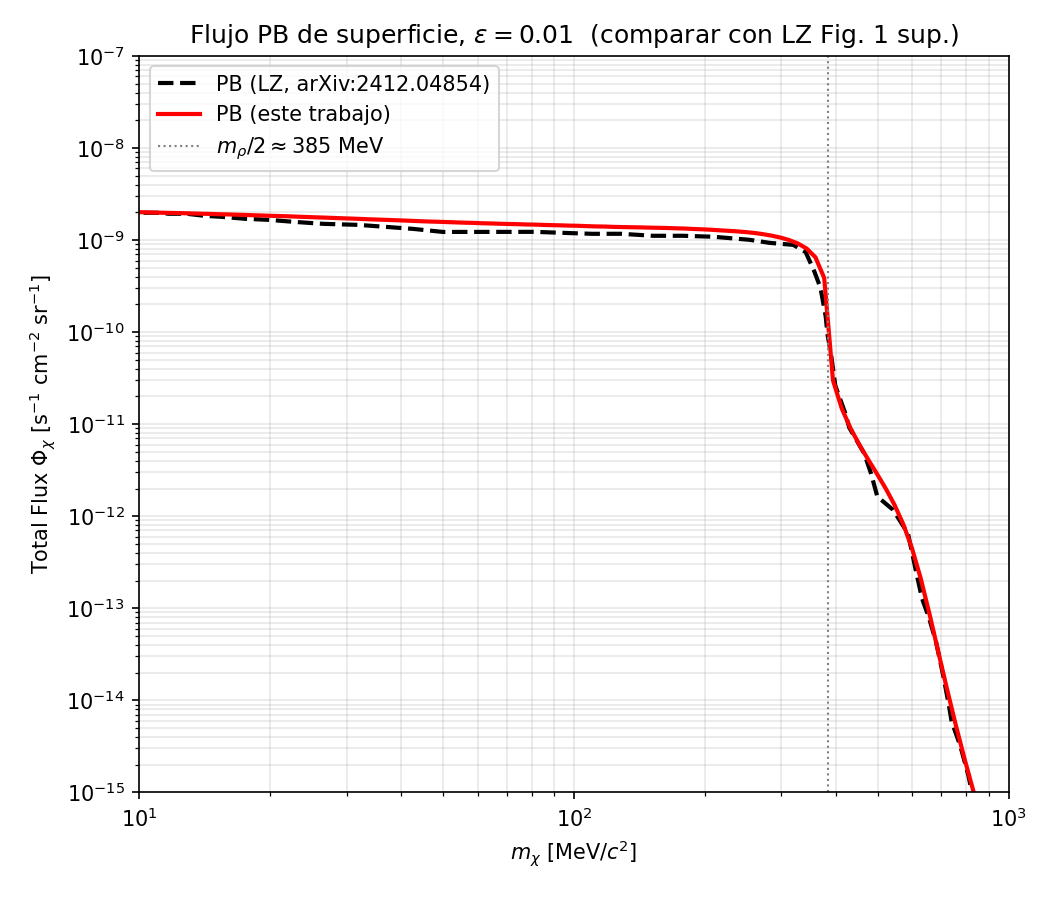
\includegraphics[width=0.72\textwidth]{LZ_PB_flux_reproduction.png}
\caption{Flujo PB de superficie integrado en energ\'ia, $\Phi_\chi^s(\mchi)$,
a $\eps=0.01$, calculado con esta implementaci\'on. Comparar con la curva PB
(roja) del panel superior de la Fig.~1 de \LZ. La l\'inea vertical punteada
marca $\mchi=m_\rho/2$, donde el umbral corta la resonancia $\rho/\omega$ y el
flujo se desploma.}
\label{fig:LZ}
\end{figure}

Algunos valores de referencia (archivo \texttt{PB\_surface\_flux\_eps0.01.csv}):

\begin{center}
\begin{tabular}{cc}
\toprule
$\mchi$ [MeV] & $\Phi_\chi^s$ [\si{cm^{-2}.s^{-1}.sr^{-1}}] \\
\midrule
10   & $2.01\times10^{-9}$ \\
100  & $1.42\times10^{-9}$ \\
275  & $1.15\times10^{-9}$ \\
331  & $8.96\times10^{-10}$ \\
398  & $2.51\times10^{-11}$ \\
575  & $7.68\times10^{-13}$ \\
1000 & $5.53\times10^{-17}$ \\
\bottomrule
\end{tabular}
\end{center}

% ============================================================
\section{Incertidumbres y puntos abiertos}
% ============================================================

La \emph{forma} de la curva (meseta $+$ codo $+$ ca\'ida) es el check m\'as
robusto y se reproduce muy bien. Sobre la \emph{normalizaci\'on absoluta}
($\sim2\times10^{-9}$ a \SI{10}{MeV}), tres factores la afectan:
\begin{itemize}
\item \textbf{$\Lambda$ (form factor off-shell)}: \Du{} indica que la
producci\'on PB fluct\'ua $\sim\!1$ orden de magnitud para
$\Lambda\in[1,2]$~GeV. Es la sistem\'atica dominante.
\item \textbf{Factor 2 ($\chi$ vs $\chi+\bar\chi$)}: implementamos la Ec.~3.1
tal cual (prefactor $\eps^2 e^2/6\pi^2$, sin factor 2 extra). En MD, \Du{}
pone un ``2'' expl\'icito por los dos mCP del par (Ec.~A.1); hay un argumento
de que el $6\pi^2$ (en vez del $12\pi^2$ natural de $\mathrm{Im}\,\Pi$) ya
incluye el par. Se debe fijar superponiendo contra \LZ.
\item \textbf{Incertidumbre propia de \LZ}: $46\%$ en el flujo PB.
\end{itemize}
Por eso un acuerdo a factor $\sim\!2$ en normalizaci\'on es satisfactorio. El
modo de cerrar el punto es digitalizar la curva roja de \LZ{} y superponer:
si el desajuste es exactamente $2\times$, el candidato es el factor
$\chi+\bar\chi$.

% ============================================================
\section{Estructura del c\'odigo}
% ============================================================

\begin{description}
\item[\texttt{pb\_splitting\_kernel.py}] Constantes; $F_V$ (Ec.~3.9),
$F_\ast$ (Ec.~3.10); \texttt{kernel\_CM} (Ecs.~3.6--3.7); boost
\texttt{cm\_to\_lab}/\texttt{lab\_to\_cm} y \texttt{s\_from\_Ep};
\texttt{kernel\_lab} (para la Fig.~5).
\item[\texttt{validate\_fig5\_du.py}] Reproduce la Fig.~5 de \Du{} (test del
kernel): imprime los endpoints cinem\'aticos y compara los Jacobianos
\texttt{full}/\texttt{kmag}/\texttt{none}.
\item[\texttt{pb\_surface\_flux.py}] Flujo de protones (Ec.~2.2); integral
interna $I$ (Ec.~\ref{eq:inner}); grilla en $k^2$ con la resonancia;
\texttt{multiplicity} (Ec.~\ref{eq:mult}); \texttt{surface\_flux}.
\item[\texttt{reproduce\_LZ\_PB\_flux.py}] Calcula $\Phi_\chi^s(\mchi)$ y
genera la Fig.~\ref{fig:LZ} y el CSV.
\end{description}

Compatibilidad: c\'odigo probado con \texttt{numpy} $<2.0$ (usa
\texttt{np.trapz}) y $\ge2.0$ (usa \texttt{np.trapezoid}, ya que
\texttt{np.trapz} fue eliminado). Se usa \texttt{np.trapz} en el entorno de
trabajo.

% ============================================================
\section{Pr\'oximos pasos}
% ============================================================

\begin{enumerate}
\item \textbf{Flujo diferencial} $\dd\Phi/\dd E_\chi$: retener la distribuci\'on
plana en $E_\chi$ (l\'imites $E_\pm=\Ek/2\pm\tfrac12\sqrt{\Ek^2-k^2}\sqrt{1-4\mchi^2/k^2}$),
necesario para atenuar.
\item \textbf{Atenuaci\'on a SNOLAB}: aplicar la Ec.~4.2 de \Du{}
($E_\chi^s=(E_\chi+a/b)e^{\eps^2 bX}-a/b$, con $a=\SI{0.233}{GeV/mwe}$),
que confirma nuestro modelo previo de p\'erdida de energ\'ia.
\item \textbf{Fijar el factor 2} contra la Fig.~1 de \LZ.
\item Sumar PB al MD y recomputar el l\'imite de exclusi\'on de SENSEI.
\end{enumerate}

\end{document}
